\section{Introduction}
\label{sec:introduction}

The current chapter covers the root of the problem and goals we are trying to accomplish.

\subsection{Motivation}
\label{sec:motivation}

Computer information analysis is the only known approach to work with huge amount of data produced every day. In any field of human work there is data and there are tasks of analyzing it. The topic of this thesis combines two areas of data computing: information visualization and biological data processing.

There are many datasets for analysis in biology. This thesis is intended to make a visualization tool for genes and gene relations in order to help biologists with their work. Data for processing was provided by the Plant Bioinformatics Group of Leibniz Institute of Plant Genetics and Crop Plant Research (IPK), Germany. Data consists of Gene Ontologies and hierarchical clustering which are are both important tools in biology and medicine for high-throughput data study.

To help analyzing this data the following approaches are desired: visualizing the data set in the context of a ontology (such as the Gene Ontology) and in the context of data clustering. There is no solutions that deals with combined visualization of ontology (DAG) and an hierarchical clustering (tree) of one data set. The aim of this work is creation of a new visualization approach and is implementation in order to provide a useful tool for biologists in their everyday research work.

The result of this work is a base of the research paper~\cite{MY_PAPER}.

\subsection{Thesis Collaboration}
This project is the result of collaboration between ISOVIS research group (Head: Prof. Dr. Andreas Kerren~\cite{Kerren}) of Linnaeus University at V\"axj\"o, Sweden, and Plant Bioinformatics Group (Head: Prof. Dr. Falk Schreiber~\cite{Schreiber}) of Leibniz Institute of Plant Genetics and Crop Plant Research (IPK), Germany.


ISOVIS research group is focused on the exploration analysis and visualization of large information data in Software Engineering, Geography, or Biology. There are several different techniques for information visualization, one of them is widely used in the research is Human-Centered Visualization. This kind of visualization combines different research areas: Information Visualization, Scientific Visualization, Human-Computer Interaction, Data Mining, Information Design, Graph Drawing, and Computer Graphics.


As said on official page of Plant Bioinformatic Group:
\begin{quotation}
``The research group focuses on modeling, analysis, simulation and visualization of biological networks in the context of plant biological problems.
Our aim is the development of methods and software tools for the analysis of complex biological networks.
Therefore we integrate, process and analyze data from different areas of genome, proteome and metabolome research and present the results in a user-friendly way.
The emphasis is on the linkage of experimental data about expression profiles and metabolite patterns with metabolic and regulatory networks.
The data and complex connections are modeled using graphs. We are developing graph (network) analysis and interactive visualization methods to discover network properties and to make the data easily accessible to the user.
A subsequent step is to use the data for the simulation of metabolic and regulatory networks.''~\cite{PBG}

Current work fulfills goals of the ISOVIS research group stated above and provides the useful tool for the researchers of the Plant Bioinformatics Group in their everyday work.

\end{quotation}


\subsection{Thesis Outline}
\label{sec:structure}

Following Section~\ref{sec:background} presents the results of the related work, where relevant research efforts in the fields of Bioinformatic, Information Visualization and Bio-Visualization were explored in connection to the thesis work. Section~\ref{sec:algorithm} covers the following topics: visualization complexity and describes the goals, description of the input data and mapping between graphs. Section~\ref{sec:solution} describes attempt to the visualization solution, the solution for Cluster Ananlysis tree and the visualization solution for Gene Ontology visualization technique. One of the biggest section in the report is Section~\ref{sec:implementation} that determines the requirements, use cases, and proposes the architecture for thesis application.
Additionally in Section~\ref{sec:solution} describes the input data format overview, overview of the different graph file formats, implementation details, architecture of the system, used libraries, project management tools. Technical details of the visualization algorithms are explained in Sections~\ref{sec:cluster} and~\ref{sec:go}. Last part of the report is Section~\ref{sec:conclusion} that describes problems and future work.

\newpage
\section{Background}

Following chapter covers the data domain we are developing for.

\label{sec:background}


\subsection{Information Visualization}
\label{sec:infovis}

\begin{quotation}
``The field of computer-based information visualization draws on ideas from several intellectual traditions:
computer science, psychology, semiotics, graphic design, cartography, and art.
The two main threads of computer science relevant for visualization are computer graphics and human-computer interaction.
The areas of cognitive and perceptual psychology offer important scientific guidance on how humans perceive visual information.
A related conceptual framework from the humanities is semiotics, the study of symbols and how they convey meaning.
Design, as the name suggests, is about the process of creating artifacts well-suited for their intended purpose.
Cartographers have a long history of creating visual representations that are carefully chosen abstractions of the real world.
Finally, artists have refined methods for conveying visual meaning in sub-disciplines ranging from painting to cinematography.''~\cite{InfoVis}
\end{quotation}

Information visualization tries to present abstract concepts and relationships that do not necessarily have a counterpart in the physical world using the graphical models. 

Application of information visualization transform and represent source data of any format (binary, textual, etc.) in such a visual form that allows human interaction. Using the interactive visualization program the data can be analyzed by exploration rather than using pure mathematical algorithms. Users the visualization program can understand the structure and connections in the data by observing the immediate effects of their interaction. 

\begin{figure}[h!]
\centering
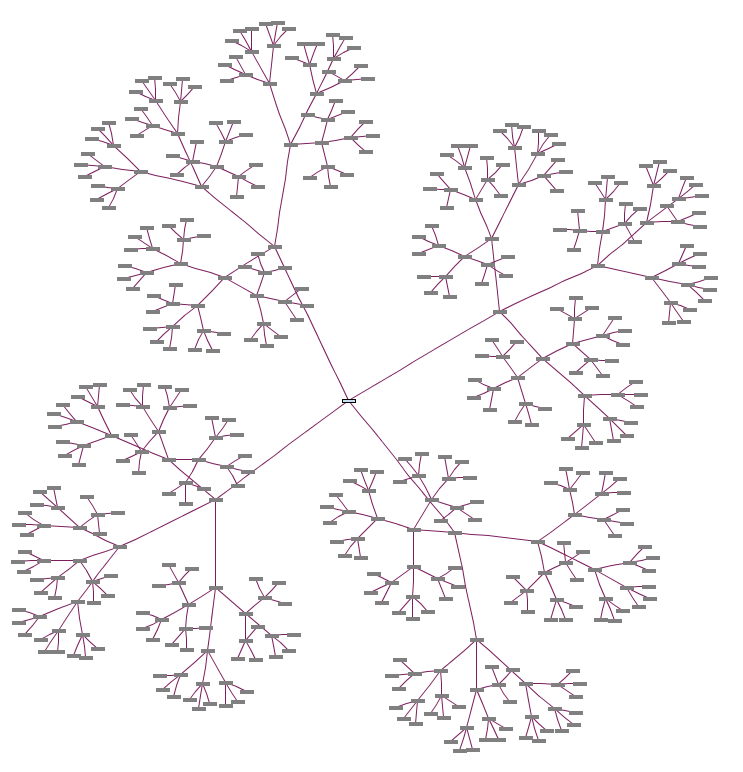
\includegraphics[scale=0.3]{pictures/Tree_graph_example.png}
\caption{Sample visualisation of the tree graph}
\label{fig:tree_graph_example}
\end{figure}

\begin{quotation}
``Graph drawing is an area of mathematics and computer science combining methods from geometric graph theory and information visualization to derive two-dimensional depictions of graphs arising from applications such as social network analysis, cartography, and bioinformatics.''~\cite{Graph_drawing}
\end{quotation}

Graph drawing algorithms varies by the type of graphs they try to represent. There are large amount of available algorithms, some of the are general purpose visualization algorithms -- to visualize any type of the graph, and the other are focused for the specific kind of graph.

In the current work we introduced two new visualization approaches based on the specific properties of the provided data. Visualization approaches will be covered in the corresponded sections. But it is worth to mention that Gene Ontology graph visualization idea is based on the Layer Graph Drawing method.

\begin{quotation}
``Layered graph drawing methods are best suited for directed acyclic graphs or graphs that are nearly acyclic, such as the graphs of dependencies between modules or functions in a software system. In these methods, the nodes of the graph are arranged into horizontal layers using methods such as the Coffman–Graham algorithm, in such a way that most edges go downwards from one layer to the next; after this step, the nodes within each layer are arranged in order to minimize crossings.''~\cite{Layered_graph_drawing}
\end{quotation}


Cluster Tree are usually represented using the dendrogram plot. The dendrogram plot is one of the visualization algorithm for hierarchical structures. It illustrating the outcome of decision tree-type clustering in statistics, in computational biology to illustrate the clustering of genes or samples~\cite{Dendrogram}

There are many methods and approaches to graph visualization. They are all based on various perception qualities of human.
The Radial Dendrograms~\cite{Radial_dendrogram} algorithm is circular layout.

\begin{quotation}
``Circular layout methods place the vertices of the graph on a circle, choosing carefully the ordering of the vertices around the circle to reduce crossings and place adjacent vertices close to each other. Edges may be drawn either as chords of the circle or as arcs inside or outside of the circle. In some cases, multiple circles may be used.''~\cite{Circular_layout}
\end{quotation}



\subsection{Bioinformatics}
\label{sec:bioinformatics}

Last years advances in molecular biology and the equipment available for research in this field have allowed the increasingly rapid sequencing of large portions of the genomes of several species.
In fact, to date, several bacterial genomes, as well as those of some simple eukaryotes (e.g., Saccharomyces cerevisiae, or baker's yeast) have been sequenced in full.
The Human Genome Project, designed to understand all twenty four genomes of the human chromosomes, is also in progress. Popular sequence databases, for example Gene Ontology project, have been growing tremendously.
This huge amount of information requires the careful storage, organization and indexing of sequence information. Information science has been applied to biology to produce the field called -- Bioinformatics.


The primary goal of bioinformatics is to increase our understanding of biological processes.


Major research efforts in the field include sequence alignment, gene finding, genome assembly, protein structure alignment, protein structure prediction, prediction of gene expression and protein-protein interactions, genome-wide association studies and the modeling of evolution.


The simplest tasks used in bioinformatics concern the creation and maintenance of databases of biological information.
Nucleic acid sequences (and the protein sequences derived from them) comprise the majority of such databases. While the storage and or organization of millions of nucleotides is far from trivial,
designing a database and developing an interface whereby researchers can both access existing information and submit new entries is only the beginning.
The most pressing tasks in bioinformatics involve the analysis of sequence information.~\cite{Biology}


Here we can find short introduction and history of Bioinformatics:

\begin{quotation}
``Bioinformatics is the application of information technology to the field of molecular biology.
The term bioinformatics was coined by Paulien Hogeweg in 1978 for the study of informatic processes in biotic systems.
Bioinformatics now entails the creation and advancement of databases, algorithms, computational and statistical techniques, and theory to solve formal and practical problems arising from the management and analysis of biological data.
Over the past few decades rapid developments in genomic and other molecular research technologies and developments in information technologies have combined to produce a tremendous amount of information related to molecular biology.
It is the name given to these mathematical and computing approaches used to glean understanding of biological processes.
Common activities in bioinformatics include mapping and analyzing DNA and protein sequences, aligning different DNA and protein sequences to compare them and creating and viewing 3D models of protein structures.''~\cite{Bioinformatic}
\end{quotation}

The developed tool helps to reach the goals of the Bioinformatics stated above through analyzing the Gene Ontology data and corresponded mappings.

More resources about Bioinformatic are available in~\cite{Bioinformatic_resources}.

\subsection{Gene Ontology}
\label{sec:gene_ontology}

As stated above, there are different knowledge databases for biologic information storage.
Gene Ontology~\cite{GO_website} project is one of the first-rate international projects.
The Gene Ontology, or GO, is a major bioinformatics initiative to unify the representation of gene and gene product attributes across all species.
The aims of the Gene Ontology project are threefold. Firstly, to maintain and further develop its controlled vocabulary of gene and gene product attributes,
secondly, to annotate genes and gene products, and assimilate and disseminate annotation data,
and thirdly, to provide tools to facilitate access to all aspects of the data provided by the Gene Ontology project. The GO is part of a larger classification effort, the Open Biomedical Ontologies (OBO)~\cite{OBO}.

In the current work one of the input data is Gene Ontology graph. The Gene Ontology is used by researchers of the Plant Bioinformatics Group to run clustering algorithm. Different goals use different algorithms as the result provides different clustering trees. GO helps to gather and share information withing researchers. Here is description from the project web-site:

\begin{quotation}
``The Gene Ontology project provides an ontology of defined terms representing gene product properties.
The ontology covers three domains.


First is cellular component and the parts of a cell or its extracellular environment.


Second is molecular function and the elemental activities of a gene product at the molecular level, such as binding or catalysis and biological process.


Finally the third are operations or sets of molecular events with a defined beginning and end, pertinent to the functioning of integrated living units: cells, tissues, organs, and organisms. Each GO term within the ontology has a term name, which may be a word or string of words;
a unique alphanumeric identifier; a definition with cited sources; and a name space indicating the domain to which it belongs.
Terms may also have synonyms, which are classed as being exactly equivalent to the term name, broader, narrower, or related; references to equivalent concepts in other databases;
and comments on term meaning or usage. The GO ontology is structured as a directed acyclic graph, where each term has defined relationships to one or more other terms in the same domain, and sometimes to other domains. The GO vocabulary is designed to be species-neutral,
and includes terms applicable to prokaryotes and eukaryotes, single and multicellular organisms.
The GO ontology is not static, therefore additions, corrections and alterations are suggested by and solicited from members of the research and annotation communities, as well as by those directly involved in the GO project.
For example, an annotator may request a specific term to represent a metabolic pathway, or a section of the ontology may be revised with the help of community experts.
Suggested edits are reviewed by the ontology editors and implemented where appropriate.''\cite{Gene_Ontology}
\end{quotation}

\subsection{Clustering}
\label{sec:clustering}

\begin{quotation}

As was mentioned in the previous section different clustering algorithm could be applied to the GO.

``Data clustering (or just clustering), also called cluster analysis, segmentation analysis, taxonomy analysis, or unsupervised classification, is a method of creating groups of objects, or clusters, in such a way that objects in one cluster are very similar and objects in different clusters are quite distinct.


Data clustering is often confused with classification, in which objects are assigned to predefined classes. In data clustering, the classes are also to be defined.''~\cite{data_clustering_book}
\end{quotation}

Clustering algorithms help to classify genes and analyze mappings between genes in the Gene Ontology graph. 


Other than in Bioinformatics and biology clustering algorithms can be applied in many other fields. For instance:

\begin{itemize}
\item Marketing: finding groups of customers with similar behavior given a large database of customer data that contains their properties and past buying records;
\item Libraries: book ordering;
\item Insurance: identifying groups of motor insurance policy holders with a high average claim cost, identifying frauds;
\item City-planning: identifying groups of houses according to their house type, value and geographical location;
\item Earthquake studies: clustering observed earthquake epicenters in order to identify dangerous zones;
\item Internet: document classification clustering web log data to discover groups of similar access patterns.
\end{itemize}